%%%% ijcai11.tex

\typeout{IJCAI-11 Instructions for Authors}

% These are the instructions for authors for IJCAI-11.
% They are the same as the ones for IJCAI-07 with superficical wording
%   changes only.

\documentclass{article}
% The file ijcai11.sty is the style file for IJCAI-11 (same as ijcai07.sty).
\usepackage{ijcai11}

% Use the postscript times font!
\usepackage{times}

% the following package is optional:

%\usepackage{latexsym} 


%\renewcommand{\baselinestretch}{.998}

%%%%%%%%%%%%%%%%%%%%%%%%%%%%%%%%%%%%%%%%%%%%%%%%%%%%%%%%%%%%%%%%%%%%%%%%
%%%%% START OF CONFIG
%%%%%%%%%%%%%%%%%%%%%%%%%%%%%%%%%%%%%%%%%%%%%%%%%%%%%%%%%%%%%%%%%%%%%%%%
\usepackage{latexsym} 
\usepackage{amsmath}
\usepackage{amssymb}
\usepackage{subfigure}
\usepackage[amssymb,thinspace]{SIunits}
\usepackage{xspace}
\usepackage{url}
\usepackage{tikz,pgf,pgfplots}
\usetikzlibrary{calc,arrows,automata,trees,shapes,plotmarks,patterns}
% You need to undefine algorithm before loading the 
% algorithm2e package, since both elsart and algorithm2e 
% define the algorithm environment.
%\makeatletter
%\newif\if@restonecol
%\makeatother
%\let\algorithm\relax
%\let\endalgorithm\relax
% Now we are ok to load algorithm2e
\usepackage[ruled,vlined]{algorithm2e}

%%%%%%%%%%%%%%%%%%%%%%%%%%%%%%%%%%%%%%%%%%%%%%%%%%%%
% PERSONAL LaTex MACROS 
%	SEBASTAN SARDINA -- ssardina@cs.rmit.edu.au
%%%%%%%%%%%%%%%%%%%%%%%%%%%%%%%%%%%%%%%%%%%%%%%%%%%%



%%%%%%%%%%%%%%%%%%%%%%%%%%%%%%%%%%%%%%%%%%%%%%%%%%%%
% Font modes & definitions
%%%%%%%%%%%%%%%%%%%%%%%%%%%%%%%%%%%%%%%%%%%%%%%%%%%%

% conditional math environment
% \gdef\Math#1{\ifmmode #1 \else \mbox{$#1$}\fi}
\newcommand{\Math}[1]{\ensuremath{#1}}



\newcommand{\modesf}[1]{{\Math{\mathsf{#1}}}}
\newcommand{\modecal}[1]{{\Math{\mathcal{#1}}}}
\newcommand{\modeit}[1]{{\Math{\mathit{#1}}}}


\newcommand{\textmath}[1]{{\mbox{\textit{#1}}}}


%%%%%%%%%%%%%%%%%%%%%%%%%%%%%%%%%%%%%%%%%%%%%%%%%%%%
% Proper names
%%%%%%%%%%%%%%%%%%%%%%%%%%%%%%%%%%%%%%%%%%%%%%%%%%%%
\newcommand{\propername}[1]{\mbox{\small \textsf{#1}}}

\newcommand{\Golog}{\propername{Golog}}
\newcommand{\GologSpeak}{\propername{GologSpeak}}
\newcommand{\DGolog}{\propername{DGolog}}
\newcommand{\sGolog}{\propername{sGolog}}
\newcommand{\ConGolog}{\propername{ConGolog}}
\newcommand{\IndiGolog}{\propername{IndiGolog}}
\newcommand{\LeGolog}{\propername{LeGolog}}
\newcommand{\DTGolog}{\propername{DTGolog}}
\newcommand{\Prolog}{\propername{Prolog}}
\newcommand{\AgentSpeak}{\propername{AgentSpeak}}
\newcommand{\JASON}{\propername{Jason}}
\newcommand{\CANMINUS}{\propername{\CAN$^{\A}$}}
\newcommand{\CANMINUST}{\propernametiny{Can$^{\cal C}$}}
\newcommand{\CAN}{\propername{CAN}}
\newcommand{\CANT}{\propernametiny{Can}}
\newcommand{\CANPLAN}{\propername{CANPlan}}
\newcommand{\CANPLANT}{\propernametiny{CanPlan}}
\newcommand{\CANPLANII}{\propername{CanPlan2}}
\newcommand{\CANPLANOR}{\propername{Can(Plan)}}
\newcommand{\CANGOAL}{\propername{CanGoal}}
\newcommand{\JACK}{\propername{Jack}}
\newcommand{\JACKTM}{\propername{Jack\texttrademark}}
\newcommand{\JAM}{\propername{JAM}}
\newcommand{\PRS}{\propername{PRS}}
\newcommand{\SPARK}{\propername{SPARK}}
\newcommand{\RAP}{\propername{Rap}}
\newcommand{\dMARS}{\propername{dMARS}}
\newcommand{\TAPL}{\propername{3APL}}
\newcommand{\DAPL}{\propername{2APL}}
\newcommand{\GOALBDI}{\propername{GOAL}}
\newcommand{\JSHOP}{\propername{JSHOP}}
\newcommand{\JSHOPII}{\propername{JSHOP2}}
\newcommand{\ASHOP}{\propername{A-SHOP}}
\newcommand{\SHOP}{\propername{SHOP}}
\newcommand{\SHOPII}{\propername{SHOP2}}
\newcommand{\ACT}{\propername{ACT}}
\newcommand{\SIPEII}{\propername{SIPE-2}}
\newcommand{\OPLANII}{\propername{O-PLAN2}}
\newcommand{\Retsina}{\propername{Retsina}}
\newcommand{\IPEM}{\propername{IPEM}}
\newcommand{\SAGE}{\propername{Sage}}
\newcommand{\DECAF}{\propername{Decaf}}
\newcommand{\PROPICE}{\propername{Propice-Plan}}
\newcommand{\CYPRESS}{\propername{Cypress}}
\newcommand{\CPEF}{\propername{CPEF}}
\newcommand{\JADEX}{\propername{JADEX}}
\newcommand{\IMPACT}{\propername{IMPACT}}
\newcommand{\PDT}{\propername{PDT}}


%%%%%%%%%%%%%%%%%%%%%%%%%%%%%%%%%%%%%%%%%%%%%%%%%%%%
% Calligraphic letters - Taken from Giuseppe De Giacomo 2006
%%%%%%%%%%%%%%%%%%%%%%%%%%%%%%%%%%%%%%%%%%%%%%%%%%%%
\newcommand{\A}{\modecal{A}} \newcommand{\B}{\modecal{B}}
\newcommand{\C}{\modecal{C}} \newcommand{\D}{\modecal{D}}
\newcommand{\E}{\modecal{E}} \newcommand{\F}{\modecal{F}}
\newcommand{\G}{\modecal{G}} \renewcommand{\H}{\modecal{H}}
\newcommand{\I}{\modecal{I}} \newcommand{\J}{\modecal{J}}
\newcommand{\K}{\modecal{K}} \renewcommand{\L}{\modecal{L}}
\newcommand{\M}{\modecal{M}} \newcommand{\N}{\modecal{N}}
\renewcommand{\O}{\modecal{O}} \renewcommand{\P}{\modecal{P}}
\renewcommand{\S}{\modecal{S}} \newcommand{\T}{\modecal{T}}
\newcommand{\U}{\modecal{U}} \newcommand{\V}{\modecal{V}}
\newcommand{\W}{\modecal{W}} \newcommand{\X}{\modecal{X}}
\newcommand{\Y}{\modecal{Y}} \newcommand{\Z}{\modecal{Z}}
\newcommand{\R}{\modecal{R}} 



%%%%%%%%%%%%%%%%%%%%%%%%%%%%%%%%%%%%%%%%%%%%%%%%%%%%
% Situation Calculus macros
%%%%%%%%%%%%%%%%%%%%%%%%%%%%%%%%%%%%%%%%%%%%%%%%%%%%

% Sitcalc Golog/ConGolog/IndiGolog programs
\newcommand{\mif}{\mbox{\bf if}}
\newcommand{\mwhile}{\mbox{\bf while}}
\newcommand{\mreturn}{\mbox{\bf return}}
\newcommand{\mthen}{\mbox{\bf then}}
\newcommand{\melse}{\mbox{\bf else}}
\newcommand{\mdo}{\mbox{\bf do}}
\newcommand{\mnoOp}{\mbox{\bf $noOp$}}
\newcommand{\mproc}{\mbox{\bf proc}}
\newcommand{\mend}{\mbox{\bf end}}
\newcommand{\mendproc}{\mbox{\bf endProc}}
\newcommand{\mendif}{\mbox{\bf endIf}}
\newcommand{\mendwhile}{\mbox{\bf endWhile}}
\newcommand{\mendfor}{\mbox{\bf endFor}}
\newcommand{\mfor}{\mbox{\bf for}}
\def\prparallel{\mathrel{\rangle\!\rangle}}
\def\supparallel{\mathord{|\!|}}
\newcommand{\conc}{\mbox{$\parallel$}}
\newcommand{\pconc}{\mbox{$\prparallel$}}
\newcommand{\search}{\mbox{$\Sigma$}}
\newcommand{\searchO}{\mbox{$\Sigma_o$}}
\newcommand{\searchOM}{\mbox{$\Sigma_o^M$}}
\newcommand{\searchCR}{\mbox{$\Sigma_{cr}$}}
\newcommand{\searchR}{\mbox{$\Sigma_{r}$}}
\newcommand{\searchM}{\mbox{$\Sigma^M$}}
\newcommand{\searchC}{\mbox{$\Sigma_c$}}
\newcommand{\searchCM}{\mbox{$\searchC^M$}}
\newcommand{\searchCB}{\mbox{$\Sigma_{cb}$}}
\newcommand{\searchD}{\mbox{$\Delta$}}
\newcommand{\searchE}{\mbox{$\Delta_e$}}
\newcommand{\searchEM}{\mbox{$\Delta_e^M$}}
\newcommand{\searchL}{\mbox{$\Delta_l$}}
\newcommand{\searchER}{\mbox{$\Delta_r$}}
\newcommand{\searchERM}{\mbox{$\Delta_r^M$}}
\newcommand{\mnt}{\mbox{$mnt$}}


%%% Knowledge in sitcalc
\newcommand{\Know}{\mbox{\bf Know}}
\newcommand{\KWhether}{\mbox{\bf KWhether}}
\newcommand{\Kref}{\mbox{\bf KRef}}
\newcommand{\nows}{{\hbox{\small\sf now}}}
\newcommand{\now}{{\mbox{\sf now}}}


% IndiGolog macros
\newcommand{\Sensed}{\textmath{Sensed}}
\newcommand{\hend}{\textmath{end}}
\newcommand{\Trans}{\textmath{Trans}}
\newcommand{\Final}{\textmath{Final}}
\newcommand{\Poss}{\textmath{Poss}}
\newcommand{\Transobs}{\textmath{TransObs}}


%%%%%%%%%%%%%%%%%%%%%%%%%%%%%%%%%%%%%%%%%%%%%%%%%%%%
% CAN notation for BDI Agents
%%%%%%%%%%%%%%%%%%%%%%%%%%%%%%%%%%%%%%%%%%%%%%%%%%%%
\newcommand{\Goal}{\modesf{Goal}}
\newcommand{\GoalS}{\modesf{G}}
\newcommand{\SGoal}{\modesf{SGoal}}
\newcommand{\SGoalS}{\modesf{SG}}
\newcommand{\goal}[3]{{\sf Goal}(#1,#3,#2)}
\newcommand{\goalp}[3]{{\sf Goal}_{P}(#1,#3,#2)}
\newcommand{\goalsfp}{\goal{s}{f}{P}}
\newcommand{\goalsfpp}{\goalp{s}{f}{P}}
\newcommand{\goalt}[2]{{\sf Goal}(#1,#2)}
\newcommand{\goalsf}{\goal{s}{f}}

\newcommand{\Plan}{\modesf{Plan}}
\newcommand{\PlanP}{\modesf{P}}
\newcommand{\PlanArg}[1]{\Plan(#1)}

\newcommand{\pnil}{\mbox{\textit{nil}}}
\newcommand{\ptrue}{\mbox{\textit{true}}}
\newcommand{\pfalse}{\mbox{\textit{false}}}
\newcommand{\pfail}{\mbox{\textit{fail}}}

\newcommand{\pguardaltl}[1]{\mbox{$\altl #1 \altr$}} % guarded alternatives
\newcommand{\altl}{\llparenthesis}
\newcommand{\altr}{\rrparenthesis}

%% Macro for BDI plan rules:  \plane{a:b<-c} \plans{a<-c}
\newcommand\plane[1]{\planeaux!#1!}
\def\planeaux!#1:#2<-#3!{\Math{#1 \mbox{\rm:} #2\; \leftarrow #3}}
\newcommand\plans[1]{\planeaux!#1!}
\def\planeaux!#1<-#2!{\Math{#1 \leftarrow #2}}




%%%%%%%%%%%%%%%%%%%%%%%%%%%%%%%%%%%%%%%%%%%%%%%%%%%%
% START - Operational semantics
%%%%%%%%%%%%%%%%%%%%%%%%%%%%%%%%%%%%%%%%%%%%%%%%%%%%
% Labels
\newcommand{\bdi}{bdi}
\newcommand{\htn}{plan}
\newcommand{\transitionlabel}[1]{\modesf{{#1}}}

% Meta-transition
\newcommand{\mtransition}{\Longrightarrow} % meta transition
\newcommand{\mtransitionstar}{\overset{*}{\mtransition}} % trans meta closure
\newcommand{\mtransitiontype}[1]{\overset{\transitionlabel{#1}}{\mtransition}}
\newcommand{\mtransitionstartype}[1]{\overset{*}{\mtransitiontype{#1}}}

% Transition
\newcommand{\transition}{\longrightarrow} 	% regular transition

\newcommand{\transitionstar}{\overset{*}{\transition}} % trans closure
\newcommand{\transitionst}{\overset{*}{\transition}} %trans closure
\newcommand{\transitionanot}[1]{\transition_{#1}} 	% regular transition
\newcommand{\transitionbdistarint}
	{\overset{\transitionlabel{\bdi}_{*}}{\transition_i}}

\newcommand{\transitiontype}[1]{\overset{\transitionlabel{#1}}{\transition}}
\newcommand{\transitionbdi}{\overset{\transitionlabel{\bdi}}{\transition}}
\newcommand{\transitionhtn}{\overset{\transitionlabel{\htn}}{\transition}}
\newcommand{\transitionhtnstar}
	{\overset{\transitionlabel{\htn}_{*}}{\transition}}
\newcommand{\transitionbdistar}
{\overset{\transitionlabel{\bdi}_{*}}{\transition}}

\newcommand{\transitionhtnk}[1]
{\overset{\transitionlabel{\htn}_{#1}}{\transition}}
\newcommand{\transitionbdik}[1]
{\overset{\transitionlabel{\bdi}_{#1}}{\transition}}



%%%%%%%%%%%%%%%%%%%%%%%%%%%%%%%%%%%%%%%%%%%%%%%%%%%%
% Several notations
%%%%%%%%%%%%%%%%%%%%%%%%%%%%%%%%%%%%%%%%%%%%%%%%%%%%

%%%%%%%%%%%%%%%%%%%%%%%%%% Delimiters
\newcommand{\quotes}[1]{{\lq\lq #1\rq\rq}}
\newcommand{\set}[1]{\{#1\}}                      % set
\newcommand{\Set}[1]{\left\{#1\right\}}
\newcommand{\bigmid}{\Big|}
\newcommand{\card}[1]{|{#1}|}                     % cardinality of a set
\newcommand{\Card}[1]{\left| #1\right|}
\newcommand{\cards}[1]{\sharp #1}
\newcommand{\sub}[1]{[#1]}
\newcommand{\tuple}[1]{\Math{\langle #1 \rangle}}		% tuple
\newcommand{\Tuple}[1]{\Math{\left\langle #1 \right\rangle}}		% tuple
\newcommand{\tup}[1]{\tuple{#1}}            			% tuple
\newcommand{\Tup}[1]{\Tuple{#1}}
\newcommand{\config}[1]{\tuple{#1}}	% configuration

% A symbol with something on top and under: \underoverset{under}{above}{text}
\newcommand{\underoverset}[3]{\underset{#1}{\overset{#2}{#3}}}


\newcommand{\myi}{\emph{(i)}\xspace}
\newcommand{\myii}{\emph{(ii)}\xspace}
\newcommand{\myiii}{\emph{(iii)}\xspace}
\newcommand{\myiv}{\emph{(iv)}\xspace}
\newcommand{\myv}{\emph{(v)}\xspace}
\newcommand{\myvi}{\emph{(vi)}\xspace}


%%%%%%%%%%%%%%%%%%%%%%%%%%%%%%%%%%%%%%%%%%%%%%%%%%%%
% Several useful symbols
%%%%%%%%%%%%%%%%%%%%%%%%%%%%%%%%%%%%%%%%%%%%%%%%%%%%

% Symbols
\newcommand{\powerset}{\mathbb{P}}
\newcommand{\NatN}{\Math{\mathbb{N}_0}} % naturals+0
\newcommand{\Nat}{\Math{\mathbb{N}}}
\newcommand{\mgu}{\modesf{mgu}}
\newcommand{\complexsub}{\modesf{cplex}}

% True and False
\newcommand{\true}{\mathtt{true}}
\newcommand{\false}{\mathtt{false}}
\newcommand{\True}{\mathtt{True}}
\newcommand{\False}{\mathtt{False}}
\newcommand{\TRUE}{\uppercase{\true}}
\newcommand{\FALSE}{\uppercase{\false}}

% LTL modalities
\newcommand{\mnext}{\bigcirc}		% next
\newcommand{\malways}{\square}		% always
\newcommand{\meventually}{\lozenge}	% eventually
\newcommand{\muntil}{\mathop{\U}}	% until

% Relations
\newcommand{\goto}[1]{\stackrel{#1}{\longrightarrow}}
\newcommand{\gotoii}[2]{\underoverset{#2}{#1}{\longrightarrow}}
\newcommand{\isdef}{\hbox{$\stackrel{\mbox{\tiny def}}{=}$}}

%%%%%%%%%%%%%%%%%%%%%%%%%%%%%%%%%%%%%%%%%%%%%%%%%%%%
% Macros for Proofs
%%%%%%%%%%%%%%%%%%%%%%%%%%%%%%%%%%%%%%%%%%%%%%%%%%%%

% Proofs symbols: provided by amsmath package now as \qed
\newcommand{\qedblack}{\phantom{a} \hfill \ensuremath{\blacksquare}}



\long\def\eatpar#1{%
\ifx#1\par                      % se il token e' \par
\let\nextmove=\eatpar           % rimetti \eatpar in coda
\else
\let\nextmove=#1%               altrimenti, rimetti il token in coda
\fi
\nextmove%                      il token o \eatpar viene rimesso in coda
}

\def\qed{\hfill{\qedboxempty}      % qed with empty box
  \ifdim\lastskip<\medskipamount \removelastskip\penalty55\medskip\fi}

\def\qedboxempty{\vbox{\hrule\hbox{\vrule\kern3pt
                 \vbox{\kern3pt\kern3pt}\kern3pt\vrule}\hrule}}

\def\qedfull{\hfill{\qedboxfull}   % qed with full box
  \ifdim\lastskip<\medskipamount \removelastskip\penalty55\medskip\fi}

\def\qedboxfull{\vrule height 4pt width 4pt depth 0pt}

\newcommand{\markfull}{\qedfull}
\newcommand{\markempty}{\qed}


%%%%%%%%%%%%%%%%%%%%%%%%%%%%%%%%%%%%%%%%%%%%%%%%%%%%
% Several special text abbreviations
%%%%%%%%%%%%%%%%%%%%%%%%%%%%%%%%%%%%%%%%%%%%%%%%%%%%

% Italic-text abbreviations (sets, etc.)
\newcommand{\CNF}{\modeit{CNF}}
\newcommand{\Actions}{\modeit{Act}}
\newcommand{\Events}{\modeit{Event}}
\newcommand{\freeVar}{\modeit{dom}}
\newcommand{\variant}{\modesf{ren}}
\newcommand{\Init}{\modeit{Init}}

\newcommand{\dummytask}{\mbox{\textit{dummyTask}}}


\newcommand{\BDI}{\mbox{BDI}}

\newcommand{\Active}{\modeit{Act}}






%%%%%%%%%%%%%%%%%%%%%%%%%%%%%%%%%%%%%%%%%%%%%%%%%%%%
% Margin notes for comments  
%%%%%%%%%%%%%%%%%%%%%%%%%%%%%%%%%%%%%%%%%%%%%%%%%%%%
\setlength{\marginparwidth}{0.8in}
\let\oldmarginpar\marginpar
\renewcommand\marginpar[1]{\-\oldmarginpar[\raggedleft\footnotesize #1]%
{\raggedright\footnotesize #1}}

% \setlength{\marginparwidth}{0.5in}
\newcommand{\notem}[1]{\marginpar{\textbf{#1}}}
\newcommand{\notetext}[1]{\notem{OBS} \textit{#1}}

\newcommand{\ncheck}{\notem{CHECK!}}
\newcommand{\GGG}{\notem{GGG}}
\newcommand{\SSS}{\notem{SSS}}
\newcommand{\LIN}{\notem{LP}}
\newcommand{\YVES}{\notem{YL}}




%%%%%%%%%%%%%%%%%%%%%%%%%%%%%%%%%%%%%%%%%%%%%%%%%%%%
% PhD boxed notes for the committee in Toronto -- Taken from Ron Petrick 2004
%%%%%%%%%%%%%%%%%%%%%%%%%%%%%%%%%%%%%%%%%%%%%%%%%%%%
% \usepackage{color}
\newcounter{countphdnote}
% \newcommand{\phdnote}[1]{\textbf{#1}}
% \newcommand{\phdnote}[1]{
% \begin{center}
% \begin{tabular}{c}
% 	\begin{minipage}{4in}
% 		\fcolorbox{black}{black}{\textcolor
%     		{white}{\textbf{\ Note \thecountphdnote\ }}}
% 	\end{minipage} \\
%     	\fcolorbox{black}{white}{
% 	\begin{minipage}{6in}
% 		#1\addtocounter{countphdnote}{1}%
%     	\end{minipage}}
% \end{tabular}
% \end{center}}



%%%%%%%%%%%%%%%%%%%%%%%%%%%%%%%%%%%%%%%%%%%%%%%%%%%%
% Tighter lists -- From Lin Padgham 2007
%%%%%%%%%%%%%%%%%%%%%%%%%%%%%%%%%%%%%%%%%%%%%%%%%%%%
\newcounter{bean}

\newenvironment{tightenumerate}{
                \begin{list}{
                  {\mbox {
                      \arabic{bean}.\/}}}{\usecounter{bean}
                      \setlength{\itemsep}{-1pt}\setlength{\topsep}{0pt}}}{
                \end{list}}

\newenvironment{tightitemize}{
                \begin{list}{$\bullet$}{
                    \setlength{\itemsep}{-1pt}}{\setlength{\topsep}{0pt}}}{
                \end{list}}
%\setlength{\itemsep}{0pt}}{\setlength{\topsep}{0pt}}}{

\renewenvironment{tightenumerate}{\begin{enumerate}}{\end{enumerate}}
\renewenvironment{tightitemize}{\begin{itemize}}{\end{itemize}}




%%%%%%%%%%%%%%%%%%%%%%%%%%%%%%%%%%%%%%%%%%%%%%%%%%%%
% General useful macros
%%%%%%%%%%%%%%%%%%%%%%%%%%%%%%%%%%%%%%%%%%%%%%%%%%%%

% Produces citations as follows: Author (Year)
\newcommand{\citeby}[1]{\citeauthor{#1} (\citeyear{#1})}

% Mark pages (pp. xxx)
\newcommand{\page}{pp.}

% Marker text
\newcommand{\marker}[1]{\textbf{******* \today: #1 *******}}

% Good underline --- Ttaken from Hector Levesque 2003
%	underline with space between text and line
\newcommand{\under}[1]{\mbox{\underline{\it\smash{#1}\vphantom{\lower.05ex\hbox{
x}}}}}

% \newcommand{\defterm}[1]{\under{\textit{#1}}}
\newcommand{\defterm}[1]{\textit{#1}}

% Comments -- just ignore everything: same as \comment{} in comment package
\newcommand{\commentarea}[1]{}

% Finish a page compactly (remove trailing space)
\newcommand{\finishpage}{ \newpage{ \pagestyle{empty} } }

% Separation for itemizations
\newcommand{\separation}[1]{\addtolength{\itemsep}{#1}}




%%%%%%%%%%%%%%%%%%%%%%%%%%%%%%%%%%%%%%%%%%%%%%%%%%%%
% Definition of Environments
%%%%%%%%%%%%%%%%%%%%%%%%%%%%%%%%%%%%%%%%%%%%%%%%%%%%

\newcommand{\finishproof}{\phantom{aaa} \hfill\ }

\newenvironment{myproof}[2]
	{\noindent {\sc Proof of #1 \ref{#2}} (\page\ \pageref{#2}):}
	{ \ \hfill \qed}

% \newenvironment{proof}
% 	{ \normalfont \noindent {\sc Proof:}}
% 	{ \qed}

% \newenvironment{proof}{\begin{proof}}{\begin{end}}
% \newtheorem{proof}{proof}
% \newenvironment{proof}[0]{\textsc{Proof.\ }\normalfont}{\qedsymbol}
\newenvironment{proofsk}{\textsc{Proof (sketch).\ }}{\qed}

% Environments
% \newtheorem{subtheorem}{Theorem}[subsection]
% \newtheorem{theorem}{Theorem}[section]
% \newtheorem{conjecture}[theorem]{Conjecture}
% \newtheorem{corollary}[theorem]{Corollary}
% \newtheorem{definition}[theorem]{Definition}
% \newtheorem{proposition}[theorem]{Proposition}
% \newtheorem{lemma}[theorem]{Lemma}
% \newtheorem{example}[theorem]{Example}
% 
% \newcommand{\Theorem}[1]{ \begin{theorem} #1 \end{theorem} }
% \newcommand{\Definition}[1]{ \begin{definition} #1 \end{definition} }
% \newcommand{\Lemma}[1]{ \begin{lemma} #1 \end{lemma} }
% \newcommand{\Claim}[1]{ \begin{claim} #1 \end{claim} }
% \newcommand{\Example}[1]{ \begin{example} #1 \end{example} }






%%%%%%%%%%%%%%%%%%%%%%%%%%%%%%%%%%%%%%%%%%%%%%%%%%%%
% EOF: macros-sebastian.tex
%%%%%%%%%%%%%%%%%%%%%%%%%%%%%%%%%%%%%%%%%%%%%%%%%%%%

\newcommand{\mathname}[1]{\operatorname{\textit{#1}}}

%%%%%%%%%%%%%%%%%%%%%%%%%%%%%%%%%%%%%%%%%%%%%%%%%%%%%%%%%%%%%%%%%%%%%%%%
%%%%% END OF CONFIG
%%%%%%%%%%%%%%%%%%%%%%%%%%%%%%%%%%%%%%%%%%%%%%%%%%%%%%%%%%%%%%%%%%%%%%%%

% Following comment is from ijcai97-submit.tex:
% The preparation of these files was supported by Schlumberger Palo Alto
% Research, AT\&T Bell Laboratories, and Morgan Kaufmann Publishers.
% Shirley Jowell, of Morgan Kaufmann Publishers, and Peter F.
% Patel-Schneider, of AT\&T Bell Laboratories collaborated on their
% preparation.

% These instructions can be modified and used in other conferences as long
% as credit to the authors and supporting agencies is retained, this notice
% is not changed, and further modification or reuse is not restricted.
% Neither Shirley Jowell nor Peter F. Patel-Schneider can be listed as
% contacts for providing assistance without their prior permission.

% To use for other conferences, change references to files and the
% conference appropriate and use other authors, contacts, publishers, and
% organizations.
% Also change the deadline and address for returning papers and the length and
% page charge instructions.
% Put where the files are available in the appropriate places.

%\setlength\titlebox{2.5in}
\title{Integrating Learning into a BDI Agent for Environments with Changing Dynamics}


% Author information can be set in various styles:
% For several authors from the same institution:
% \author{Author 1 \and ... \and Author n \\
%         Address line \\ ... \\ Address line}
% if the names do not fit well on one line use
% \author{Author 1 \\ {\bf Author 2} \\ ... \\ {\bf Author n} \\
%         Address line \\ ... \\ Address line}
% For authors from different institutions:
% \author{Author 1 \\ Address line \\  ... \\ Address line
%         \And  ... \And
%         Author n \\ Address line \\ ... \\ Address line}
% To start a separate ``row'' of authors use \AND, as in
% \author{Author 1 \\ Address line \\  ... \\ Address line
%         \AND
%         Author 2 \\ Address line \\ ... \\ Address line \And
%         Author 3 \\ Address line \\ ... \\ Address line}

% If the title and author information does not fit in the area allocated,
% place \setlength\titlebox{<new height>} after the \documentstyle line
% where <new height> is something like 2.5in
\author{
Dhirendra Singh, Sebastian Sardina, Lin Padgham\\
RMIT University\\
Melbourne, Australia\\
{\normalsize\{dhirendra.singh,sebastian.sardina,lin.padgham\}@rmit.edu.au}
\And
Geoff James\\
CSIRO Energy Technology\\
Sydney, Australia\\
{\normalsize geoff.james@csiro.au}
}

%\author{Dhirendra Singh\inst{1} \and Sebastian Sardina\inst{1} \and Lin Padgham\inst{1} \and Geoff James\inst{2}
%\institute{
%\inst{1}School of Computer Science \& Information Technology\\College of Science Engineering and Health\\RMIT University
%\and
%\inst{2}CSIRO Energy Technology
%}
%}


\begin{document}

\maketitle

\begin{abstract}
%Belief, Desire, and Intentions (BDI) agent-oriented programming is a popular 
%paradigm for developing complex applications that are able to deal
%with multiple ways of achieving goals, depending on the situation. 
%BDI systems rely on \emph{plan libraries} to achieve
%\emph{goals}, and on \emph{context sensitive} subgoal selection and
%expansion. 
%
An important drawback to the popular Belief, Desire, and Intentions
(BDI) paradigm is that such systems include no
element of learning from experience. Plans, and conditions under
which they should be selected, are determined at
design/implementation. 
%This precludes the system adapting to a
%changing environment that has not been foreseen.
%
Another limitation is that although there may be mechanisms for 
establishing preferences, applicability of plans is generally
regarded as a binary decision. 
%They are either applicable to the
%current context, or not. although there may be some mechanism for
%recording or establishing preferences.
% 
In this work we replace formula based context conditions with decision
trees, to represent world states in which
the plan is likely to succeed or fail, with some level of probability.
The decision tree, and associated estimates of success/failure,
changes based on experience. We use a probabilistic plan selection function
that allows us to balance exploration and exploitation in selection of
plans.
%
We develop and empirically investigate an aggressive and a
conservative approach to learning context conditions, showing that
both can be advantageous in certain situations. In particular the
aggressive approach can at times be too agressive, leading to complete
inability to learn.
%
We then develop a more sophisticated plan selection approach which
takes account of how much we have explored, and therefore to what
extent we should rely on our estimate of success. We show that this
successfully addresses the problems associated with aggressive
learning sometimes ruling out options too readily, and thus never
learning correct behaviour.
% 
We empirically evaluate our approaches on a range of
different program structures.


\end{abstract}

%%%%%%%%%%%%%%%%%%%%%%%%%%%%%%%%%%%%%%%%%%%%%%%%%%%%

%!TEX root = ../ijcai11storage.tex
% %%%%%%%%%%%%%%%%%%%%%%%%%%%%%%%%%%%%%%%%%%%%%%%%%%%
\section{Introduction}\label{sec:introduction}
% %%%%%%%%%%%%%%%%%%%%%%%%%%%%%%%%%%%%%%%%%%%%%%%%%%%


The Belief-Desire-Intentions (BDI) agent programming paradigm
\cite{WooldridgeBook,BusettaRHL:AL99-JACK,Pokahr:EXP03-JADEX,jasonbook} is a
successful and popular approach to developing complex systems that
behave robustly in situations where the environment is
interacting with the system.
However, BDI agents do not incorporate learning, and once deployed,
have no ability to adjust to changes in the dynamics of an environment
that cause previously successful approaches to fail and vice versa.
%%
In this work we maintain the structure and advantages of a BDI agent
program, but integrate adaptive machine
learning techniques that are generally used to learn behaviour in a
fixed environment (often off-line with a training set),
for use in online continuous learning in an environment where what
works, may well change over time.
%%
In that way, our contribution is to agent programming---\emph{to make BDI programs more adaptive by seamlessly integrating learning techniques}---rather that to machine learning research.
%%
The aim is to use the operational knowledge encoded in the agent program, but learn refinements to it so as to cope with changes in the dynamics of the environment. 

A key issue when learning is that of exploitation \emph{vs.} exploration: how much to trust and exploit the current
(learnt) knowledge, versus how much to try things in order to gain new
knowledge. 
%Important in this balance is an understanding of how much
%knowledge has already been
%explored. 
In our earlier work~\cite{singh10:extending,singh10:learning}, a
``coverage-based" measure of confidence was used to capture how much
the BDI agent should trust its current understanding (of good plan
selection), and therefore exploit rather than explore. Intuitively,
this confidence was based on the degree to which the space of possible
execution options for the plan has been explored (covered).
The more this space has been explored, the
greater the confidence, and the more likely the agent is
to exploit.   
%
As recognised in this work, the coverage-based
confidence approach does not support learning in a changing
environment. This is because the confidence increases
\emph{monotonically} and, as a result, there is no ability for the
agent to become less confident in its choices, even if its currently
learned behaviour becomes less successful due to changes in the
environment. 

Consider a smart building equipped with a large
battery system that can be charged when there is excess power, and
used (discharged) when there is excess demand, in order to
achieve an overall desired building consumption rate for some
period. A battery installation is built from independent modules with
different chemistries. Initially, the embedded battery controller can
be programmed (or can learn) to operate optimally. However, over time
modules may operate less well or even
cease to function altogether. In addition, modules may be replaced
with some frequency.   
%%	
Thus, what is needed is a controller that, after having explored
the space well and developed high confidence in its learning,
is able to observe when learned knowledge becomes unstable, and
dynamically modify its confidence allowing for new exploration and
revised learning in an ongoing way. To achieve this we develop a
confidence measure based on an assessment of how well informed our
selections are, combined with an observation of the extent to which we
are seeing new situations.

The rest of the paper is as follows.
%
First, we introduce BDI systems and machine learning
concepts necessary to understand this work.  
%
We then describe our BDI learning framework, initially developed
in~\cite{airiau09:enhancing,singh10:extending,singh10:learning}, and
extend this with our new confidence measure (Section~\ref{sec:confidence})
for learning in environments with changing dynamics.  
%
Next, we describe a battery controller agent, based on a real
application that requires ongoing learning, and show how it adjusts in
a variety of ways to an environment where battery behaviour changes.  
%
We conclude with related work and limitations requiring future work.



%\newpage
%In this work, we develop a new confidence measure, compatible with the BDI learning framework, which allows the agent to adjust its confidence as the environment changes.
%%%
%The new metric is built from two ingredients.
%%%
%First, it uses the notion of plan stability from~\cite{airiau09:enhancing,singh10:learning} to quickly estimate how much the different options for achieving a goal have been explored.
%%%
%Second, it considers how much the agent is experiencing states that have been seen before vs how much it is seeing new situations, by using a sliding window that checks what percentage of situations in the window have been seen previously. If a substantial number of new situations are being experienced, then the agent should be less confident in what it has previously learnt. 

%The rest of the paper is organised as follows.
%%%
%In the following section, we provide an overview of the basic BDI learning framework on which this work is based, as developed by~\cite{airiau09:enhancing,singh10:extending,singh10:learning}. 
%%%
%We then explain in detail our new proposal for a dynamic measure of confidence that may be used by the BDI agent at plan-selection time to continually adjust to a changing world. 
%%%
%Following that, we describe an energy storage domain taken from a real application where the environment dynamics changes over time requiring adaptive learning. We then specify some experiments evaluating the battery controller agent in different situations, and demonstrate that our learning approach for BDI systems does in fact allow the agent to adjust in a variety of ways to an environment where battery behaviour changes. 
%%%
%We conclude the paper by discussing related work and some limitations requiring future work.
%
%

%%%%%%%%%%%%%%%%%%%%%%%%%%%%%%%%%%%%%%%%%%%%%%%%%%%%
\section{Preliminaries}\label{sec:preliminaries}
%%%%%%%%%%%%%%%%%%%%%%%%%%%%%%%%%%%%%%%%%%%%%%%%%%%%

\newcommand{\success}{\mbox{\emph{succ}}}
\newcommand{\failure}{\mbox{\emph{fail}}}

\newcommand{\procedurefont}[1]{\mathsf{#1}}
\newcommand{\StableGoal}{\procedurefont{StableGoal}}
\newcommand{\RecordTrace}{\procedurefont{RecordFailedTrace}}
\newcommand{\RecordWorldDT}{\procedurefont{RecordWorldDT}}



%%%%%%%%%%%%%%%%%%%%%%%%%%%%%%%%%%%%%%%%%%%%%%%%%%%%
\subsection{BDI Agent Systems}\label{sec:bdi_programming}
%%%%%%%%%%%%%%%%%%%%%%%%%%%%%%%%%%%%%%%%%%%%%%%%%%%%

%\notems{new para}
BDI agent-oriented programming is a popular, well-studied, and practical paradigm
for building intelligent agents situated in complex and dynamic environments with
(soft) real-time reasoning and control requirements
\cite{Georgeff89-PRS,Benfield:AAMAS06}.
% %
Generally speaking, BDI agent-oriented programming languages are built
around an 
explicit representation of propositional attitudes (e.g., beliefs, desires,
intentions, etc.). A BDI architecture addresses how these components are
represented, updated, and processed to determine the agent's actions.
% .
%There are a number of agent programming languages and development platforms in
%the BDI tradition, some examples of which include
% \PRS~\cite{IngrandGR:IEEE92-PRS} and
% \dMARS~\cite{Inverno:JAAMAS04-dMARS}, \AgentSpeak\ and
%\JASON~\cite{Bordini:07-JASONBOOK},
%Rao:LNCS96-AgentSpeak,
%\JADEX~\cite{PokahrBL:EXP03-JADEX}, and
% \TAPL~\cite{Hindriks:JAAMAS99-3APL,DastaniRM:05} and
% \DAPL~\cite{Dastani:JAAMAS08-2APL}, \GOAL~\cite{BoerHHM:JAPL07-GOAL},
%\JACK~\cite{BusettaRHL:AL99-JACK}.
%, SRI's \SPARK~\cite{MorelyM:AAMAS04-SPARK}, and
%\JAM~\cite{Huber:AGENTS99-JAM}.
%ABOVE SAID IN INTRO


\begin{figure}[t]
\begin{center}
\resizebox{.7\textwidth}{!}{\begin{tikzpicture}

\tikzstyle{centityd}=[draw=black]
\tikzstyle{centityf}=[fill=black!20]
\tikzstyle{centity}=[centityd,centityf]
\tikzstyle{entity}=[centity,thick,text centered,anchor=center]


\node[anchor=east] at (6,4.5)  {dynamic};
\node[anchor=west] at (7,4.5) {static};


\node (database) at (1,8.8)  (B)
	[cylinder,entity,shape border rotate=90,minimum width=1.6cm,shape aspect=.3]
	{\textbf{Beliefs}};


\node  (environment)  
       [below left of=B, rounded corners, minimum height=3cm,
       starburst,fill=black!10,rotate=90,shift={(-1cm,4cm)}] 
       {\textbf{\large Environment}};



\node at (4,10) (eventQueue) {{\bf Pending Events}};
\begin{pgfonlayer}{foreground}
\foreach \x in {3.5,3.7,...,4.5}
\draw [fill=black!50](\x,9.2) circle (0.2);
\end{pgfonlayer}
%\path (4,9.1) node (Q) {}; 
\draw (4,9.2) node (Q) 
	[entity, text width=1.4cm, minimum height=0.8cm] {};




\foreach \x in {4,3,2,1}
\draw (-.6,5) node (I) [anchor=south,draw, centity, text width=.5em,
	minimum height=\x em]{};
\foreach \x in {3,2,1}
\draw (0.2,5) node (I) [anchor=south,draw,centity, text width=.5em,
	minimum height=\x em]{};
\foreach \x in {5,4,3,2,1}
\draw (1,5) node (I) [anchor=south,draw, centity, text width=0.5em,
	minimum height=\x em]{};
\node[below left of=I] (Intentions) {{\bf  Intention Stacks}};


% { [start chain=1]
% % \node [on chain,draw] at (0,6) {};
%     \foreach \x in {1,2,...,11} {
%        \x, \node [draw,on chain=1] {};
%     }
% }

\begin{pgfonlayer}{foreground}
\node[anchor=center] at (4,6)  (deli) 
	{\begin{tabular}{c}
     	\textbf{BDI engine} 
     \end{tabular}};
\node at (4,3.4) (actions) {{\bf actions}};
\node at (2.5,11.4) [starburst,centityd] (in) {{\bf events}};


\draw node (P) 
	[right of=deli,xshift=3cm,rounded corners, double copy
	shadow={opacity=0.8},text centered, entity, minimum height=5em] 
	{	\begin{tabular}{c} 
          \textbf{Plan} \\[1ex]
          \textbf{library}
         \end{tabular}	};



\draw[thick,->] (in) -- (B) ; 
\draw[thick,->] (in) -- (eventQueue) ; 
\draw[thick,->] (deli) -- (actions) ; 
\draw[thick,<->] (deli) -- (I) ; 
\draw[thick,<->] (deli) -- (B) ; 
\draw[thick,<-] (deli) -- (P) ;
\draw[thick,<->] (deli) -- (Q) ; 
\end{pgfonlayer}








\begin{pgfonlayer}{background}

%% Dotted box encapuslating the agent
\path (-1.5,10.5) node (c) {};
\path (9.5,4) node (d) {};
\path[fill=none,rounded corners, draw=black!50, dashed] (c) rectangle (d);




\draw[->,very thick,dashed] (environment) 
		|- node[above,xshift=1cm] {SENSORS}
	 	(in);
\draw[->,very thick,dashed] (actions.west) 
		-| node[below,xshift=1cm] {ACTUATORS}
		(environment.west);
\end{pgfonlayer}


\foreach \x in {-9,9,...,360}
\fill [rotate around={\x:(3.2,5.6)},centityf] 
	(4.0,5.4743) -- (4.2 ,5.6) -- (4.0,5.7257) -- (4.0,5.3487);
\fill [centityf] (3.2,5.6) circle (0.8);

\foreach \x in {0,18,...,360}
\fill [rotate around={\x:(4.8,6.4)},centityf] 
	(5.6,6.2743)-- (5.8,6.4) -- (5.6,6.5257) -- (5.6,6.2743);
\fill [centityf] (4.8,6.4) circle (0.8);


\end{tikzpicture}}
\end{center}
\caption{A typical BDI-style architecture}
\label{fig:bdiarch}
\end{figure}

A BDI agent consists, basically, of a belief base (akin to a
database) which stores the agent's knowledge about the world, a set of
pending events, which includes both external percepts or messages and
internal goals, a plan library and an intention structure.
% %
Figure~\ref{fig:bdiarch} depicts a typical BDI architecture.
% %
The plan library contains rules of the form $e: \psi \leftarrow
\delta$ indicating that $\delta$ is a suitable procedure for achieving
event-goal $e$ when context condition $\psi$ is true.
% %
%\notems{UAV example}
%For example, a BDI controller for an unmanned aerial vehicle (UAV)
%\cite{Karim:AAMAS05,Ziming:AAC07} may include a certain procedure $\delta$ for
%achieving the goal of \emph{landing the aircraft} (the event) under \emph{normal
%weather conditions} (the context).
% %
Among other operations, the plan body procedure $\delta$ will
typically include the 
execution of actions ($act$) in the environment and subgoal events ($!e$) that
are in turn resolved by selecting suitable plans for that subgoal
event.
%
The intention structure contains the current, partially instantiated,
plans that the agent has committed to in order to handle or
achieve some event-goals.

The basic \emph{reactive goal-oriented behavior} of BDI systems involves the
system responding to events by 
selecting an appropriate plan from the library, and placing its
program body into the intention base.
% %%
A plan is appropriate if it is designed for the event in question
(relevant) and its context
condition is believed true (applicable).
% %
In contrast with traditional planning, execution happens at each step. The
use of plans' context-preconditions to make choices as
late as possible, together with the built-in goal-failure mechanisms, ensures
that the system is responsive to changes in the environment.

%\notems{fixes in para}
In this paper we focus on the plan library to
investigate ways of learning appropriate or better plan selection
based on experience. 
% %
By grouping together plans responding to the same
event type, the plan library can be seen as a set of \emph{goal-plan tree}
templates: a goal (or event) node has children representing the alternative
relevant plans for achieving it; and a plan node, in turn, has children nodes
representing the subgoals (including primitive actions) of the plan.
% %%
These structures can be seen as AND/OR trees: for a plan to succeed all the
subgoals and actions of the plan must be successful (AND); for a subgoal to
succeed one of the plans to achieve it must succeed (OR).

\begin{figure}[t]
\begin{center}
\input{figs/gpt-example}
\end{center}
\caption{An Example BDI Goal-Plan Hierarchy.}
\label{fig:T3}
\end{figure}

Consider, for instance, the hierarachical structure shown in Figure~\ref{fig:T3}.
% %%
A link from a goal to a plan means that this plan is relevant (i.e., potentially
suitable) for achieving the goal (e.g., $P_1 \ldots P4$ are the relevant plans
for event goal $G$); whereas a link from a plan to a goal means that the plan
needs to achieve that goal as part of its (sequential) execution (e.g., plan
$P_A$ needs to achieve goal $G_{A1}$ first and then $G_{A2}$).
% %
For compactness, an edge with a label $\times n$ states that there are $n$ edges
of such type.
% %
Leaf plans directly interact with the environment and so, in a given world state,
they can either succeed or fail when executed; this is marked accordingly in the
figure \emph{for some particular world} (of course, in other states, such plans
may behave differently).
% %
In some world, given successful completion of $G_A$ first, the agent may achieve
goal $G_B$ by selecting and executing $P_B$, followed by selecting and executing two working leaf plans to resolve goals $G_{B1}$ and $G_{B2}$. If the agent
succeeds with goals $G_{B1}$ and $G_{B2}$, then it succeeds for plan $P_B$,
achieving thus goal $G_B$ and the top-level goal $G$ itself. There is no possible
successful execution though, if the agent decides to carry on any of the three
plans labelled $P_{B2}'$ for achieving the low-level goal $G_{B2}$.


As can be seen \textit{plan-selection} is critically important.
Standard BDI systems leverage domain
expertise by means of the context conditions of plans.
% However, crafting fully
%correct context conditions at design-time can, in some applications, be a
%demanding and error-prone task. In addition, fixed context conditions do not
%allow agents to adapt to changing environments.
% %%
%\notems{changed last sentence} 
In this work, we are interested in exploring how a situated agent may
\emph{learn} plan selection based on experience, in order to improve goal
achievement. 


%%%%%%%%%%%%%%%%%%%%%%%%%%%%%%%%%%%%%%%%%%%%%%%%%%%%
\subsection{Learning for BDI Plan Selection} \label{subsec:bdi_learning}
%%%%%%%%%%%%%%%%%%%%%%%%%%%%%%%%%%%%%%%%%%%%%%%%%%%%
In order to facilitate learning regarding which plan should be
executed for a given goal in a particular world state, we first replace the
boolean formulae that are the standard representation for context
conditions in BDI programming languages, with decision
trees~\cite{Mitchell97:ML} that provide a judgement as to whether the
plan is likely to succeed or fail for the given situation. 

To select a plan, based on information in the decision trees, we use a
probabilistic selection method whereby we choose a plan with
probability proportional to its believed chance of success in the
particular world state. This approach provides a balance between
exploitation (we choose plans with relatively higher success expectations
more often), and exploration (we choose plans randomly to get better
confidence in their believed success by trying them in more 
situations).

The resolution of goals in BDI execution results in 
the invocation of plans that in turn may post sub-goals that are further
handled by sub-plans in a hierarchical manner. In a programming context,
this is equivalent to making a function call that in turn calls sub-functions.
%The key difference is that the choice of sub-plans in the BDI context is
%not determined by the designer 
%% ABOVE IS NOT CORRECT
However a sub-goal may have a number of possible plans for achieving
it, some of which will work better in particular situations than
others. In our learning context, where we do not yet know which plans
work well in which situations, a plan may fail not because the plan
was a bad choice in the given situation, but instead because the
run-time choice of sub-plans was incorrect for the situation.

%As we have reported in earlier work~\cite{Airiau:IJAT:09} there are
%potential problems with learning the wrong information if a plan fails
%due to a wrong decision further down in the goal plan
%hierarchy. Consider the goal-plan tree in figure \ref{fig:bdiarch}: if
%as discussed previously we picked one of the  plans indicated by
%$P_{B2}'$ to address goal 
%$G_{B2}$ (in the world which this tree is annotated for), then we
%would fail. This failure of $G_{B2}$\footnote{We are not currently
%using BDI failure recovery.} would then cause $P_B$ to fail, failing
%$G_B$, and in turn $P_i$. As $P_{B2}'$ is a leaf node it is clearly
%reasonable to learn that this plan fails in the particular world
%state. However it is not so clear that one wants to learn that the
%parent plans $P_B$ and $P_i$ fail. In fact, as we can see in this
%annotated figure, had we made a different choice for achieving
%$G_{B2}$ they would have succeeded. If one does not take account of
%the hierarchical nature of the goal plan in some way, then it may be
%that learning is severely impacted or even made impossible.

%Our experimentation has shown that the degree to which the learning is
%negatively affected due to wrong decisions is very dependent on
%the particular structure of the goal-plan tree (i.e. the
%program). In particular, if there is a threshhold below which a plan
%is not considered worth trying (for example, if belief of success is
%only 10\%, then the cost of trying the plan may not be justified),
%then storing failure information when its reliability is unceratin,
%can lead the agent to be unable to ever learn the successful
%execution. 

Our first approach~\cite{Airiau:IJAT:09} to address this problem was that 
of careful consideration whereby failures are recorded for learning purposes 
only when we are sufficiently sure that the failure was not due to poor
sub-plan choices. 
%This requires recording which choices we have made at each
%point, for every world situation. 
We have shown that this conservative approach is more robust, 
though often slower, than a more agressive
approach which records all experiences, but can in some particular cases
completely fail to learn.

Our second approach reported in~\cite{Singh:AAMAS10} was to
adjust the plan selection probability based on some measure of 
our confidence in the decision tree classification.
%
We consider the reliability of a \dt\ for a given plan in a given 
world state to be proportional to the number of sub-plan choices (or paths
below the plan in the goal-plan hierarchy) that have been
\textit{covered} in that  
world state. The greater the coverage, the more we have explored and the
greater the confidence in the resulting \dt.
%
By biasing the plan selection probability with a coverage-based confidence
measure we achieved the same robustness as that of conservative recording of 
failure cases. The coverage approach, however, is more 
flexible as the extent to which this is used can be
readily adjusted by parameters in the selection formula. 

%A limitation with both the above
%approaches is that we have not considered parameterised goals. 
%A robot goal to move, for instance, 
%would typically have some parameters, either a destination (where the
%world state contains the current position), or a direction. Clearly a
%goal to move from A to B will require different choices than a goal to
%move from A to C (assuming B and C are not close). The learning
%process must take account of this. A second limitation is that we
%have not allowed for recursion, which again is heavily used in many
%real applications. 

A limitation with the previous approaches is that 
events were assumed to be propositional atoms, that is, event
types were not considered. By \emph{event type} we mean an event that may
contain ``data'' as part of its definition. For instance, event
$\textmath{travelTo(?dest)}$ may represent the goal to travel to location
$\textmath{?dest}$. Presumably a goal to move to location $A$ would 
require different choices than a goal to move to $B$, and the learning
must account for this.
% % 
Another limitation is the assumption that the agent's plan library is
non-recursive, so that the goal-plan tree structure induced is always
\emph{finite}.
% %
Clearly both limitations would preclude the applicability of the approach in
many practical domains where hierarchies are usually expressed
using parameterised goal events and plans, and often make
use of (direct or indirect) recursive procedures.


%Unfortunately, when we applied our previous
%coverage measures to unfolded recursive structures (with a fixed
%recursion depth), the method, which relied on exact calculation of
%numbers of paths, was no longer viable computationally, and even had
%problems conceptually. Consequently, in this and ongoing work we adopt
%an approximate measure of complexity of the goal-plan tree beneath a
%given plan and use this, combined with a graduated reliance on the
%decision tree depending on both experience and complexity of the tree
%- a more complex tree requiring more experience before we should feel
%confident of learned results.

Furthermore, the coverage approach of~\cite{Singh:AAMAS10} does not scale
when recursive structures and event-goal types are
introduced. Conceptually we can unfold the recursive structure to a
specified depth. However, the number of paths is exponential in the
recursion number and the problem is further compounded by event-goal
types and the number of possible world states.
%
An additional limitation with the
coverage-based confidence measure is that it does not consider domain
complexity. For instance, a leaf plan that has no sub-goals will
achieve full coverage when it is tried once, after which selection
will be fully biased towards the plans \dt\ classification. However,
the \dt\ that at this point has only witnessed one world will
generalise the outcome to all as-yet-unseen worlds leading to
misclassification errors. 

In the following section we present the details of our learning
approach, incorporating both parametrised goals, and recursion, as
well as a new simpler confidence measure that is based on the 
general idea of coverage but does not suffer from its limitations.








%%%%%%%%%%%%%%%%%%%%%%%%%%%%%%%%%%%%%%%%%%%%%%%%%%%%
\section{A BDI Learning Framework}\label{sec:framework}
%%%%%%%%%%%%%%%%%%%%%%%%%%%%%%%%%%%%%%%%%%%%%%%%%%%%


The problem that we are interested in is as follows: \emph{given past execution
data and the current world state, determine which plan to execute next 
in order to address an event}.


To address this ``learnable'' plan-selection task, we start by modeling the
context condition of plans with \emph{decision trees}, rather than with logical
formulas.\footnote{The logical formulae of the classical BDI framework can of course be combined with \dt s.}
% %
Decision trees~\cite{Mitchell97:ML}  provide a natural classification mechanism
for our purposes, as they can deal well with noise (generally due to partially
observable and predictable environments), and they are able to support
disjunctive hypotheses. They are also readily convertible to rules, which are the
standard representation for context conditions in BDI systems.


We associate each plan in the agent's library with a \dt\ that classifies world
states into an expectation of whether the plan will succeed or fail. Then for
each relevant plan, its \dt\ (induced based on previous executions)
gives the agent information regarding how likely it is to succeed/fail in a
particular world state.


Given this new context for BDI programming, there are two issues that ought to be
addressed.
% %%%
First, one has to decide \emph{when and what kind of execution data the agent should
collect in order to be able to ``learn'' (useful) decision trees for plans}.
Roughly speaking, data is collected regarding whether a plan is considered to
have succeeded or failed in the world for which it was selected.
% %
  Whereas successful executions are always recorded, the recording of failure
runs of a plan may be subject to some analysis; this is the topic of the following section.



The second issue to be addressed is how to use the plans' decision trees for plan
selection. More concretely: \emph{given a goal to be resolved and a set of
relevant plans with their corresponding context decision trees, what plan should
the agent commit for execution?}
% %%
Typical BDI platforms offer various mechanisms for plan selection, including plan
precedence and meta-level reasoning. However, these mechanisms are pre-programmed
and do not take into account the experience of the agent.
% %
In our framework for context learning, we must consider the standard dilemma of
\emph{exploitation} vs \emph{exploration}. To that end, we use an 
approach in which plans are selected with a probability proportional to their relative expected
success (in the world state of interest). Later, in
Section~\ref{sec:coverage}, we discuss how to further enhance such plan selection
by considering how much each candidate plan has been
explored relative to its ``complexity.''



For the purpose of our analysis, we have used algorithm
\propername{J48}, a version of \propername{c4.5} \cite{Mitchell97:ML}, from the
well-known \weka\ learning package \cite{weka99}. Currently we
recreate decision trees from scratch after each new outcome is recorded.
% %
Of course, for a real-world implementation, one should appeal to algorithms for
\emph{incremental} induction of the decision tree, such as those described in
\cite{Swere06:Fast,Utgoff97Decision}.
% %

The \weka\ \propername{J48} algorithm for inducing \dt{}s aims to balance
compactness of representation with accuracy. Consequently, it maintains in each
\dt\ information about the number of instances (or world states in our case) from
the training data correctly and incorrectly classified by each decision tree leaf
node. Subsequently, whenever a plan's \dt\ is used to classify a new instance
(world state), weka returns not only the classification (i.e. success or
failure), but also a classification probability (i.e. to what degree it believes
that the classification is correct). We then use this probability as an estimate
of the plan's chances of success for the world in question.


Finally, we should point out a number of assumptions that were made in order to
focus on the core issues we are concerned with.
% %
First, we assume that actions in the environment may fail with some probability
(if an action is not possible in a world state this probability is $1.0$).
% %
% DSINGH#1: Based on review comments, Dhirendra changed this:
%Second, we assume no external changes in the environment during execution other
%than those made by the agent. Although this may appear too limiting, the fact
%that actions may fail with some probability mitigates against
%over-simplification by capturing external changes as
%non-deterministic failures.
% DSINGH#1: to this:
This is a simple way to capture non-deterministic failures caused either by 
imperfect execution or external changes in the environment. A success on the
other hand is always attributed only to the agent's actions.
% DSINGH#1: end change
% %
Second, we consider the execution of a single intention; learning in the context
of multiple, possibly interacting, intentions poses other extra challenges that
would complicate our study substantially (see \cite{Thangarajah02}).
% % %
Lastly, we assume no automated failure handling, whereby the BDI system retries
a goal with alternative options if the selected plan happens to fail. 
% DSINGH#2: Based on review comments, Dhirendra changed this:
%Integrating failure handling would not alter any of our results, but it would
%complicate our implementation framework and the understanding of the basic
%mechanisms.
% DSINGH#2: to this:
Integrating failure handling would complicate our implementation framework and the understanding of the basic mechanisms. For instance, if an alternative plan were to succeed after the initial failure then care must be taken in propagating this outcome to the parent as the success may have been caused precisely because the first choice failed in a way that enabled the second one to succeed.
% DSINGH#2: end change




%!TEX root = ../aamas11storage.tex
% %%%%%%%%%%%%%%%%%%%%%%%%%%%%%%%%%%%%%%%%%%%%%%%%%%%
\section{A Modular Storage Application}\label{sec:introduction}
% %%%%%%%%%%%%%%%%%%%%%%%%%%%%%%%%%%%%%%%%%%%%%%%%%%%

Energy storage helps to enable increasing levels of renewable energy in our electricity system, and the rapidly maturing supply chains for several battery technologies encourages electricity utilities, generators, and customers to consider using large battery systems.  Large battery systems usually comprise multiple modules and in many installations these may be controlled independently.  Modules may be operated in synchrony but often there are strategic reasons to keep some modules in a different state to others.  For example, if it is undesirable to change the direction of power flow between charging and discharging too frequently, a subset of modules may be used for each direction until it is necessary to change their roles.  Also, some technologies have specific requirements, such as the zinc-bromine flow battery for which a complete discharge at regular intervals is desirable to �strip� the zinc plating and ensure irregularities never have an opportunity to accumulate.  Where they exist these requirements place further constraints on module control.
 
Given, then, an input signal which is the requested rate of charging and discharging for a large battery installation, as a function of time, we would like a control algorithm for the set of component modules that implements the requested rate as the sum over the module rates of charging and discharging.  The input signal will be different every day but will have many features that are diurnal or nearly so, due to typical variations of electricity demand and solar and wind energy generation sources, and the repetitive patterns that may be seen over several days of the input signal suggest that a learning algorithm may be appropriate.  Our problem is to develop a method for on-line learning that will result in a useful control regime for a modular battery system, when installed at a new site and provided with an input signal derived from the electricity demand and renewable supply at that site.

\begin{figure}[ht]
\begin{center}
%!TEX root = ./dp7-application.tex
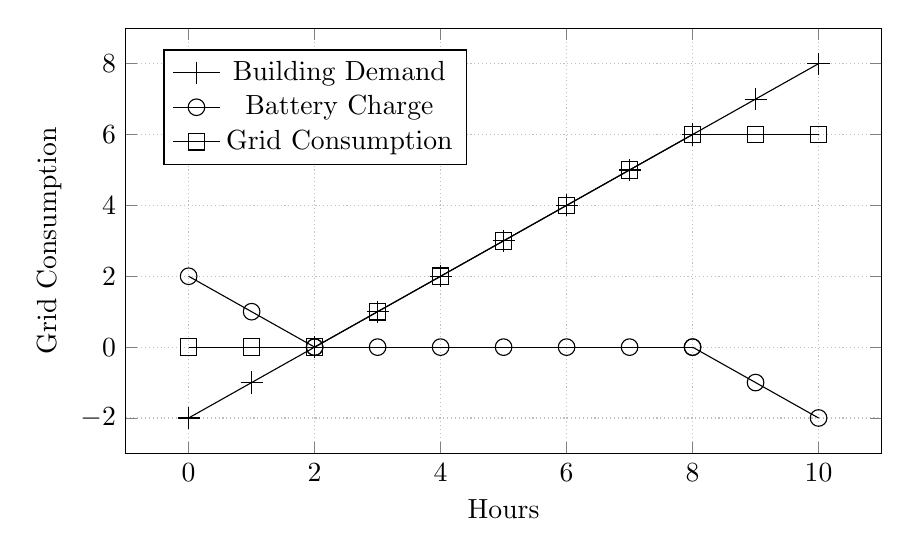
\begin{tikzpicture}

\begin{axis}[
x=0.8cm,y=0.45cm,
xlabel=Hours,
ylabel=Grid Consumption,
grid=both, grid style={style=densely dotted},
legend style={at={(0.05,0.95)},anchor=north west}
] 

% Draw the Demand-Supply curve
\addplot[mark=+,mark size=4] expression[domain=0:10,samples=11] {x-2};
\addlegendentry{Building Demand} 

% Draw the Battery curve
\addplot[mark=o,mark size=3] expression[forget plot,domain=0:2,samples=3] {2-x}; 
\addplot[mark=o,mark size=3] expression[forget plot,domain=2:8,samples=7] {0}; 
\addplot[mark=o,mark size=3] expression[domain=8:10,samples=3] {8-x}; 
\addlegendentry{Battery Charge} 

% Draw the Grid supply curve
\addplot[mark=square,mark size=3] expression[forget plot,domain=0:2,samples=3] {0}; 
\addplot[mark=square,mark size=3] expression[forget plot,domain=2:8,samples=7] {x-2}; 
\addplot[mark=square,mark size=3] expression[domain=8:10,samples=3] {6}; 
\addlegendentry{Grid Consumption} 
\end{axis} 
\end{tikzpicture} 

\end{center}
\caption{Use case scenario for the battery system during a $10$ hour period. The aim is to maintain grid consumption within the range $[0:6]$ units. Building Demand is the sum of individual loads and renewable generation and may therefore fall outside this range. By suitably ordering the charge or discharge of the battery system (Battery Charge signal), the net consumption (Grid Consumption signal) of the system may be maintained within range.}
\label{fig:usecase}
\end{figure}


\begin{figure*}[ht]
\begin{center}
%!TEX root = ../ijcai11storage.tex
\begin{tikzpicture} [level distance=5.5em,child anchor=north]
\tikzstyle{planbox}=[draw,fill=white,text width=5.1em,rectangle split,rectangle split parts=3]
\tikzstyle{goalbox}=[draw,rounded corners=1.25em,minimum height=3em,minimum width=3em]

	
\tikzstyle{level 1}=[sibling distance=6.5em] 
\tikzstyle{level 2}=[level distance=5.5em] 

\node[goalbox,solid] {$G($r,k,s$)$}
	child {node[planbox] {$\pSetCharge$ \\
			\nodepart{second} $k>0$ \\ $\cSatisfies_{ch}(r,k,s)$
			\nodepart{third} $\aSet(k,+c)$
		}
		child {node[goalbox] {$G($r,k-1,s'$)$}}
	}
	child {node[planbox] {$\pSetDischarge$ \\ 
			\nodepart{second} $k>0$ \\ $\cSatisfies_{dc}(r,k,s)$
			\nodepart{third} $\aSet(k,-c)$
		}
		child {node[goalbox] {$G($r,k-1,s'$)$}}
	}
	child {node[planbox] {$\pSetNotUsed$ \\
			\nodepart{second} $k>0$ \\ $\cSatisfies_0(r,k,s)$
			\nodepart{third} $\aSet(k,0)$
		}
		child {node[goalbox] {$G($r,k-1,s'$)$}}
	}
	child {node[planbox] {$\pExecute$ 
			\nodepart{second} $k=0$
			\nodepart{third} $\aOperate()$ \\$\aEvaluate()$
		}
	}
;

\end{tikzpicture}



\end{center}
\caption{Goal-plan hierarchy for the battery system with $k$ modules.}
\label{fig:gptree}
\end{figure*}

Consider the example scenario of a smart office building that consists of a set of individual loads (appliances in the building), some renewable generators (solar panels on the roof and a local wind turbine), and a modular battery system. The building is connected to the main grid, and the economics govern that the grid power consumption of the building be maintained within the range $[0:6]$. Since there is little control over the demand in the building and certainly no control over the renewable generation, then for some period in the day it is possible that the power consumption of the building will fall outside this range. For instance, if the renewable generation is higher than the demand, then the consumption will be negative. Similarly, if the demand is higher than the renewable generation then the building consumption may rise above $P$. In Figure \ref{fig:usecase} the Building Demand curve shows the sum of consumption and generation in the building for a $10$ hour window some given day.

While there is little control over the consumption and generation in the building (Building Demand), we do have full control over how the battery system is used. So for instance, by suitably ordering the battery system to charge (act as a load) or discharge (act as a generator) at determined rates throughout the period we may influence the net demand in the building. Figure \ref{fig:usecase} shows how the appropriate battery response (Battery Charge curve) added to the building consumption and generation (Building Demand curve) ensures that the power drawn from the grid (Grid Consumption) is maintained within the desired range.

% %%%%%%%%%%%%%%%%%%%%%%%%%%%%%%%%%%%%%%%%%%%%%%%%%%%
\subsection{Modular Storage Controller}\label{subsec:controller}
% %%%%%%%%%%%%%%%%%%%%%%%%%%%%%%%%%%%%%%%%%%%%%%%%%%%

The battery system consists of a number of internal modules that may all have individual constraints. Moreover, the charge/discharge characteristics of the modules may change over time. As such, it is desirable that the battery control algorithm be able to adapt to these changes over time. Figure \ref{fig:gptree} shows a possible learning BDI agent controller for a battery system with $k$ modules. 

The top level goal $G(k,s)$ is posted by the system at the beginning of each period of deliberation. The controller then responds by operating the battery modules for that period in a suitable configuration that resolves the goal. The parameter $k$ is initially set to the number of modules in the system\footnote{Note that the battery design may contain more internal modules than the advertised number to provide for a operational buffer. In this case the parameter $k$ should reflect this actual count.}.  The parameter $s$ specifies the desired response from the system and lies in the normalised range $[-1.0:+1.0]$ where $-1.0$ indicates a maximum discharge rate and $+1.0$ indicates a maximum charge rate.

The resolution of the battery system determines how closely it can match the desired response and depends on the number of modules $n$. For simplicity, we will assume homogeneous capacity of the modules (but with possibly different chemical properties and constraints), such that each module has a capacity $c$ and $c*n=1.0$. Each internal module in turn may be in one of three states: charging (i.e $+c$), discharging (i.e. $-c$) or not in use (i.e. $0$). The sum of these values gives the net response of the system. In other words, the response of the battery system may be adjusted in multiples of $c$.

The BDI controller works by recursively setting the operational state of each module in the system using the $Set*$ plans, and then finally running the selected configuration for one period and evaluating the result using the $Execute$ plan. The execution therefore always consists of the selection of $k$ high level $Set*$ plans followed by the $Execute$ leaf plan. Using the BDI learning framework from \cite{Singh:RAS10} the pass/fail result is then recorded in the chain of active $Set*$ plans. By training over the outcomes of each plan selection in each situation, the system over time learns correct plan selection at each recursive level for the set of possible top-level requests.


Each plan in the goal-plan hierarchy is further explained below:

$SetCharge$: Plan to set the operational state of module $k$ to {\em Charge} for this period. The plan first checks that the internal constraints of module $k>0$ will not be violated by this operation. If a violation is expected, then the plan is aborted, otherwise the state is updated and Goal $G$ reposted for module $k-1$.

$SetDischarge$: Plan to set the operational state of module $k$ to {\em Discharge} for this period. The plan first checks that the internal constraints of module $k>0$ will not be violated by this operation. If a violation is expected, then the plan is aborted, otherwise the state is updated and Goal $G$ reposted for module $k-1$.

$SetNotUsed$: Plan to set the operational state of module $k$ to {\em NotUsed} for this period. This means that the module will remain disconnected from use for this period. The plan first checks that the internal constraints of module $k>0$ will not be violated by this operation. If a violation is expected, then the plan is aborted, otherwise the state is updated and the Goal $G$ reposted for module $k-1$.

$Execute$: The leaf plan that actually performs the operations on the battery modules. The plan operates only when $k=0$ which implies that all modules have been configured. The battery modules are then operated for this period according to their assigned states. At the end of the period, the plan will evaluate the battery response against the goal and determine the $Pass$ or $Fail$ status. Normally, a pass would mean that the actual battery response was within tolerance of the desired response. 


The $Set*$ plans in the hierarchy may fail when selected if the constraints for module $k$ are violated for that period. For instance, plan $SetCharge$ might fail because module $k$ is only allowed to change charge directions once every four periods say, and charging it in this period will violate that constraint. Similarly, plan $SetDischarge$ might fail because the module may have critically low charge and further discharge for a full period is not possible. Finally, plan $SetNotUsed$ might fail because the module has a requirement to be fully discharged once every day, and disconnecting it in this period will violate that constraint. 

Since violation checks are performed prior to taking any action, then BDI failure recovery may be performed to select a different $Set*$ plan until all internal constraints are satisfied prior to execution. Note that failure recovery is not allowed for the $Execute$ plan because it runs for a full period and that is the limit for the decision making. In other words, only one try is allowed per period. So functionally, the $Execute$ plan must always succeed, even though the evaluation against the goal (for learning purposes) may differ.

Finally, the system only learns a response to the immediate request i.e. how to resolve the top level goal. It does not learn any temporal relationship in the sequence of top level goals. For instance, the input signal may have some diurnal pattern, however the proposed system does not attempt to learn this pattern.

\subsection{Implementation Notes}

The system is (purposely) similar in design to the Towers of Hanoi problem of \cite{Singh:RAS10}. In some respects, it is simpler because the solutions are always at recursive depth $k$. Moreover, the non-leaf $Set*$ plans do not have side-effects when they fail and leave the initial state unaltered. Finally, a solution always consists of a single $Execute$ action whereas in the Hanoi problem it consists of possibly several $Move$ actions\footnote{One point of difference is that this is not a universal library where a solution can always be found. For some requests, no solution will be possible given the internal state of the modules.}.

Nonetheless, the problem captures a real world problem where it is not straightforward to hand-craft a functional hierarchy and where learning is justified. We do not have a solution to begin with. Then, the size of the problem is still significant - the flow battery in CSIRO Newcastle has $10$ internal modules, so with three possible module states that represents $3^{10}=59049$ possible configurations for a given request. Finally, it offers a realistic scenario for re-learning a solution due to significant changes in the environment. For instance, if an internal module were to fail and had to be replaced, then prior learning may no longer work effectively, and the system will have to adjust and re-learn it's response based on the new characteristics of the updated module.


%%%%%%%%%%%%%%%%%%%%%%%%%%%%%%%%%%%%%%%%%%%%%%%%%%%%
\section{Discussion and Conclusion}\label{sec:discussion}
%%%%%%%%%%%%%%%%%%%%%%%%%%%%%%%%%%%%%%%%%%%%%%%%%%%%

In this paper, we proposed a technique to enhance the typical plan selection
mechanism in BDI systems by allowing agents to learn and adapt the context
conditions of plans in the agent's plan library.
% %
As designing adequate context conditions that take full account of the agent's
environment for its complete life-cycle is an non-trivial task, a framework that
allows for the \emph{refinement} of (initial) context conditions of plans
\textit{based on online experience} is highly desirable.
% %
To this end, we extended the typical BDI programming framework to use \dt{}s as
(part of) plan's context conditions and provided a probabilistic plan selection
mechanism that caters for both exploration and exploitation of plans.
% %
After empirically evaluating different learning strategies suitable for BDI
agents against various kind of plan libraries, we concluded that an aggressive
learning approach combined with plan selection scheme that uses a confidence
measure based on the notion of plan coverage is the best candidate for the
general setting.
% %
The work carried out here is significant for the BDI agent-oriented programming
community, in that it provides a solid foundations for going beyond the standard
static kind of BDI agents.


The framework presented here made a number of simplifying assumptions.
% %
Our experiments did not consider the effects of conflicting interactions between
sub-goals of a plan. In fact, the way a sub-goal is resolved may affect how the
next sub-goal can be addressed or even if it can be resolved at all.
% %
Our current implementation is not possible to detect and learn such interactions;
each subgoal is treated ``locally.'' To handle such interactions, the selection
of a plan for a resolving sub-goal should also be predicated the goals higher
than the sub-goal, that is, it should take into account the ``reasons'' for the
sub-goal.
% %
Similarly, we did not consider the effects of using goal failure recovery, under
which alternative plans for a goal are tried upon the failure of a plan.
% %
Also, we have only dealt with domains described via boolean propositions. To
handle continuous attributes (e.g., discretize \emph{temperature}), our approach
requires that either these attributes are discretized or additional discrete
attributes be used to test the continuous ones (e.g., \emph{cold}, \emph{warm},
and \emph{hot}).
% %
% Lastly, we point out that even though we have used environments with a simple
% stochastic model, our results apply trivially to agents acting in environments
% based on more complex models.


One critique of the coverage-based confidence measure used is that it has a
defined end state, namely $c_T(w)=1$. In a real system, however, learning and
re-learning will occur indefinitely, as the agent continually tries to
\emph{adapt} to a changing environment. This implies that an agent's confidence
in a \dt's classification would also require calibration when the environment has
changed. If the change was deliberate, then our confidence could be reset and
subsequently \textit{re-built}. Without such an explicit signal, the agent must
rely on other methods for determining when the environment has changed
significantly.
% %
An appealing measure for recognising environmental changes is through the
relatedness of its features. For instance, an observation that the grass is
\textit{wet} may have a high correlation to the fact that it is \textit{raining}.
If at some point, the agent were to witness a world where it is not raining but
the grass is indeed wet (for some other new reasons), then this world would be
``atypical,''  and as a result, the agent may have reason to reduce its
confidence in a plan's \dt\ classification of this new world.
% %
It turns out that efficient algorithms exist---some already included in the
\weka\ library---that perform inference in and learning of Bayesian networks
\cite{Mitchell97:ML}, which the agent can appeal to build a model of the
environment for the purposes just described.



The issue of combining learning and deliberative approaches for decision making
in autonomous systems has not been widely addressed.
% %
In~\cite{Riedmiller01}, learning is used \emph{prior to deployment} for acquiring
low level robot soccer skills that are then treated as fixed methods in the
deliberative decision making process once deployed.
% %
Hern\'andez et al. \cite{Hernandez04:Learning} give a preliminary account of how
decision trees may be induced on plan failures in order to find an alternative
logical context conditions in a deterministic paint-world example.
% %
More recently, \cite{Zhuo09:Learning} proposes a method for learning hierarchical
task network (HTN) method preconditions under partial observations. There, a set
of  constraints are constructed from observed decomposition trees that are then
solved \emph{offline} using a constraint solver. Despite HTN systems being
automated planning frameworks, rather than execution frameworks, these are highly
related to BDI agent systems when it comes to the \emph{know-how} information
used---learning methods' preconditions amounts to learning plan's context
conditions.
% %
In constrast, in our work, learning and deliberation are fully integrated in a
way that one impacts the other and the classical exploration/exploitation dilemma
applies.
% Initially, instead of following a random exploration policy (as is the case for
% agents with no initial knowledge), our agents are guided by the existing domain
% knowledge inherent in the BDI hierarchy.





%%%%%%%%%%%%%%%%%%%%%%%%%%%%%%%%%%%%%%%%%%%%%%%%%%%%

\small
%% The file named.bst is a bibliography style file for BibTeX 0.99c
\bibliographystyle{named}
\bibliography{ijcai11storage}

\end{document}

